% !TEX root = template.tex

\newcommand\mygather{\texttt{MY\_Gather}\xspace}
\newcommand\myscatter{\texttt{MY\_Scatter}\xspace}

\newcommand\mpigather{\texttt{MPI\_Gather}\xspace}
\newcommand\mpiscatter{\texttt{MPI\_Scatter}\xspace}

%----------------------------------------------------------------------
\section{Algorithm \mygather}

%-------
\subsection{Strategy Comparison}

\subsubsection{Binomial Tree}

\subsubsection{Divide-And-Conquer}

%-------
\subsection{Description / Strategy}



%-------
\subsection{Round- and Bandwidth Optimality}

%-------
\subsection{Harmful Algorithmic Latency}

%----------------------------------------------------------------------
\section{Algorithm \myscatter}

%-------
\subsection{Strategy Comparison}

\subsubsection{Binomial Tree}

\subsubsection{Divide-And-Conquer}

%-------
\subsection{Description / Strategy}

%-------
\subsection{Round- and Bandwidth Optimality}

%-------
\subsection{Harmful Algorithmic Latency}

%----------------------------------------------------------------------
\section{Experimental Results}

%-------
\subsection{Experiments and Discussion -- \mygather}

\begin{figure}[h]
    \centering
    
    \begin{subfigure}[b]{0.49\textwidth}
        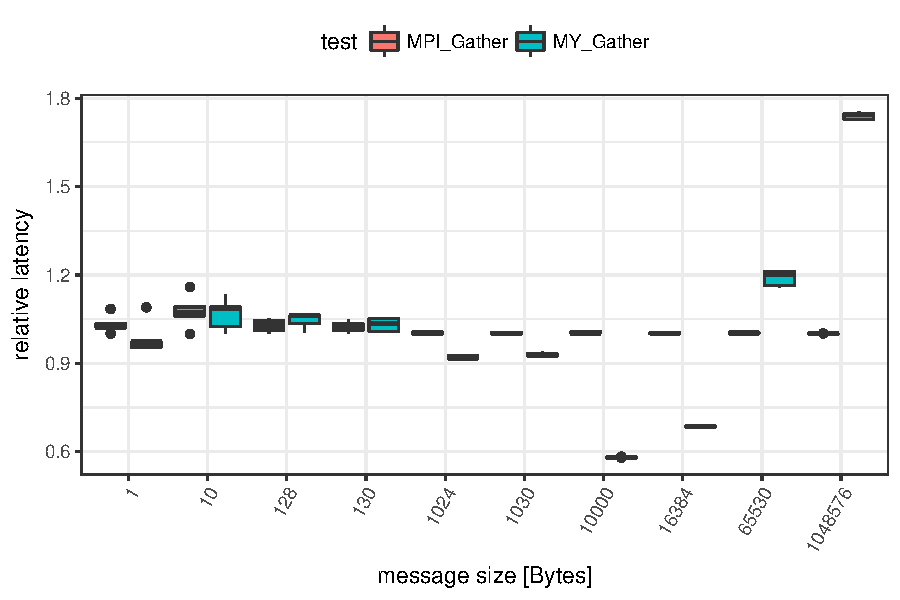
\includegraphics[width=\textwidth]{../benchmarks/openmpi/binom/gather_31/rel_runtime.pdf}
        \caption{Relative Runtime with $p=31 \times 16$}
        \label{fig:Gather:OpenMPI:Rel:31}
    \end{subfigure}
    \begin{subfigure}[b]{0.49\textwidth}
        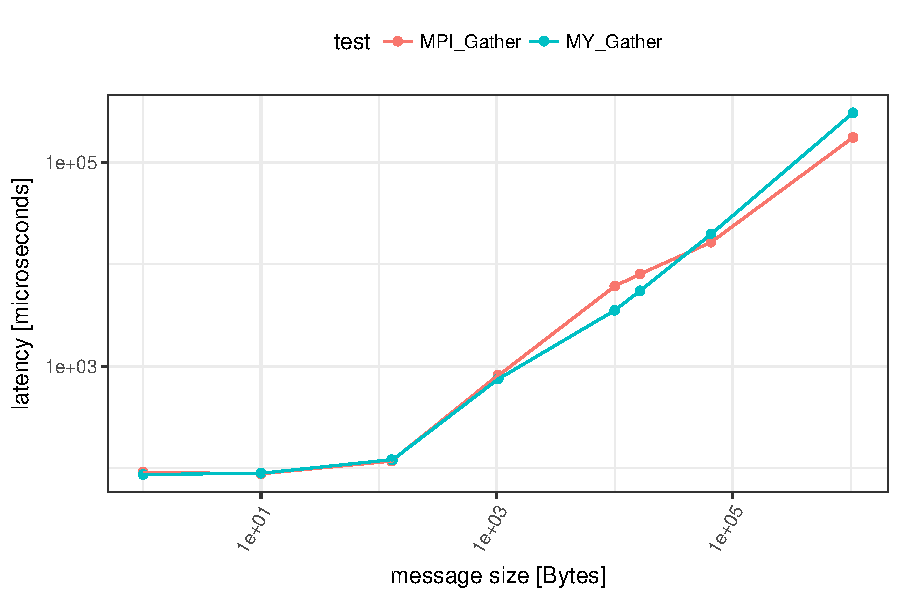
\includegraphics[width=\textwidth]{../benchmarks/openmpi/binom/gather_31/runtime.pdf}
        \caption{Absolute Runtime with $p=31 \times 16$}
        \label{fig:Gather:OpenMPI:Abs:31}
    \end{subfigure}
    
    \begin{subfigure}[b]{0.49\textwidth}
        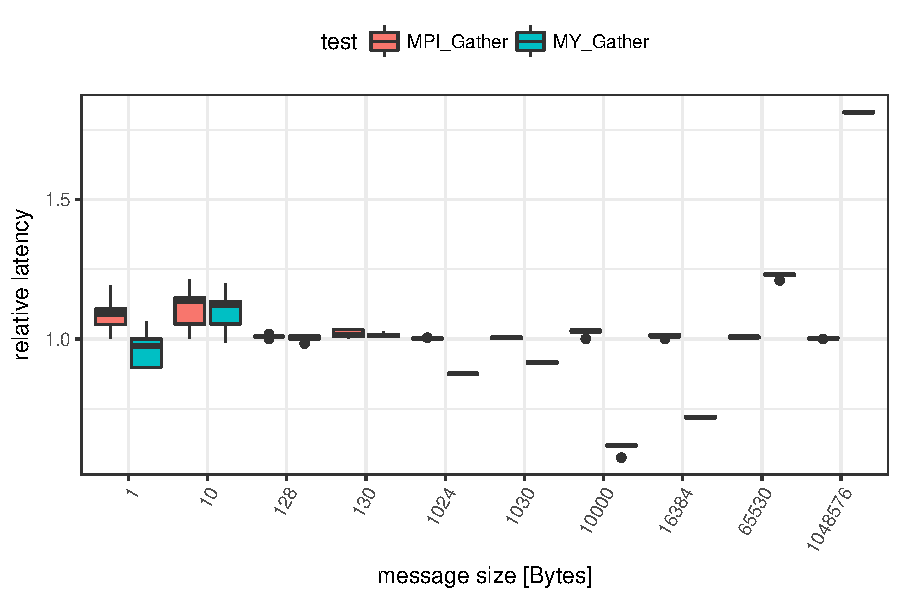
\includegraphics[width=\textwidth]{../benchmarks/openmpi/binom/gather_32/rel_runtime.pdf}
        \caption{Relative Runtime with $p=32 \times 16$}
        \label{fig:Gather:OpenMPI:Rel:32}
    \end{subfigure}
    \begin{subfigure}[b]{0.49\textwidth}
        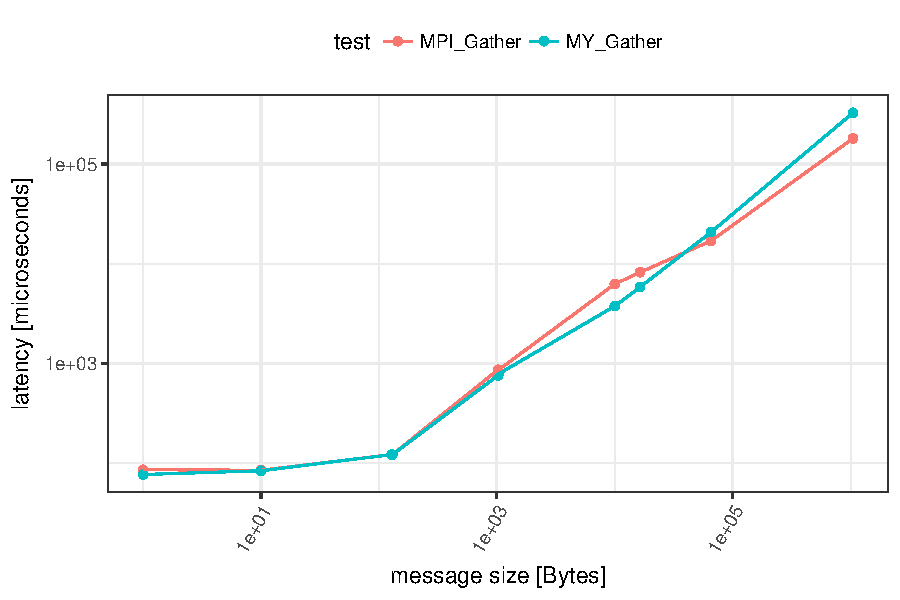
\includegraphics[width=\textwidth]{../benchmarks/openmpi/binom/gather_32/runtime.pdf}
        \caption{Absolute Runtime with $p=32 \times 16$}
        \label{fig:Gather:OpenMPI:Abs:32}
    \end{subfigure}
    
    \caption{\mygather compared to \mpigather of \texttt{Open MPI 1.10.3}}
\end{figure}

\begin{figure}[h]
    \centering
    
    \begin{subfigure}[b]{0.49\textwidth}
        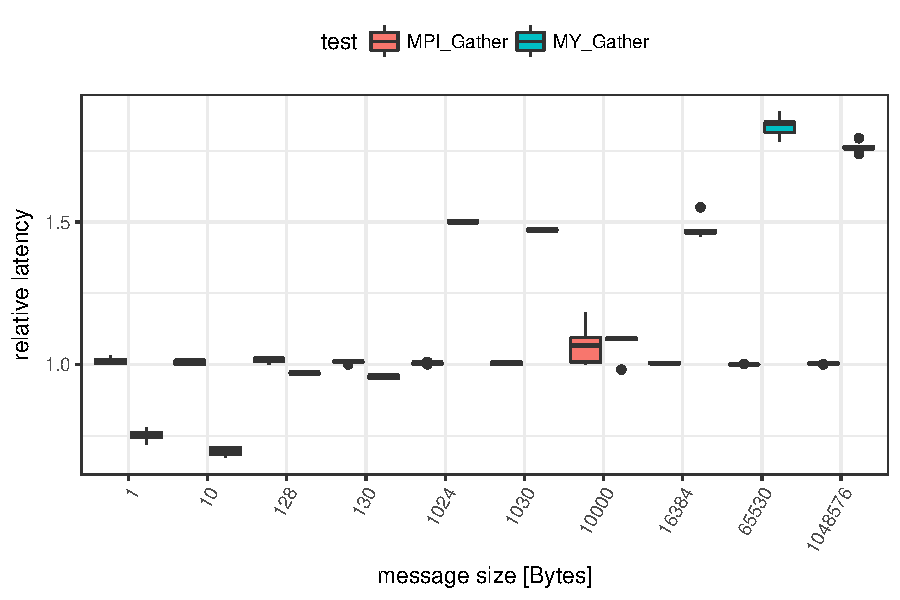
\includegraphics[width=\textwidth]{../benchmarks/mpich/binom/gather_31/rel_runtime.pdf}
        \caption{Relative Runtime with $p=31 \times 16$}
        \label{fig:Gather:MPICH:Rel:31}
    \end{subfigure}
    \begin{subfigure}[b]{0.49\textwidth}
        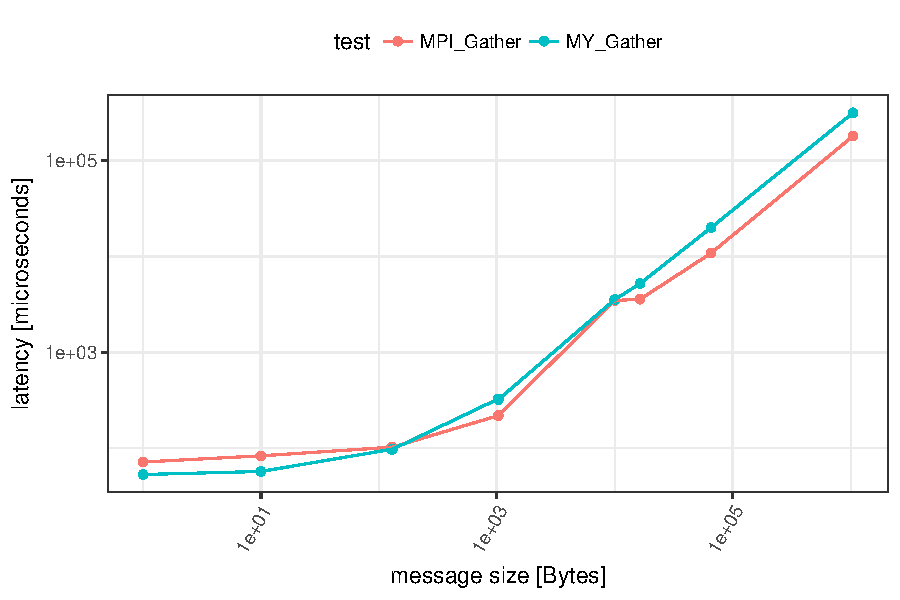
\includegraphics[width=\textwidth]{../benchmarks/mpich/binom/gather_31/runtime.pdf}
        \caption{Absolute Runtime with $p=31 \times 16$}
        \label{fig:Gather:MPICH:Abs:31}
    \end{subfigure}
    
    \begin{subfigure}[b]{0.49\textwidth}
        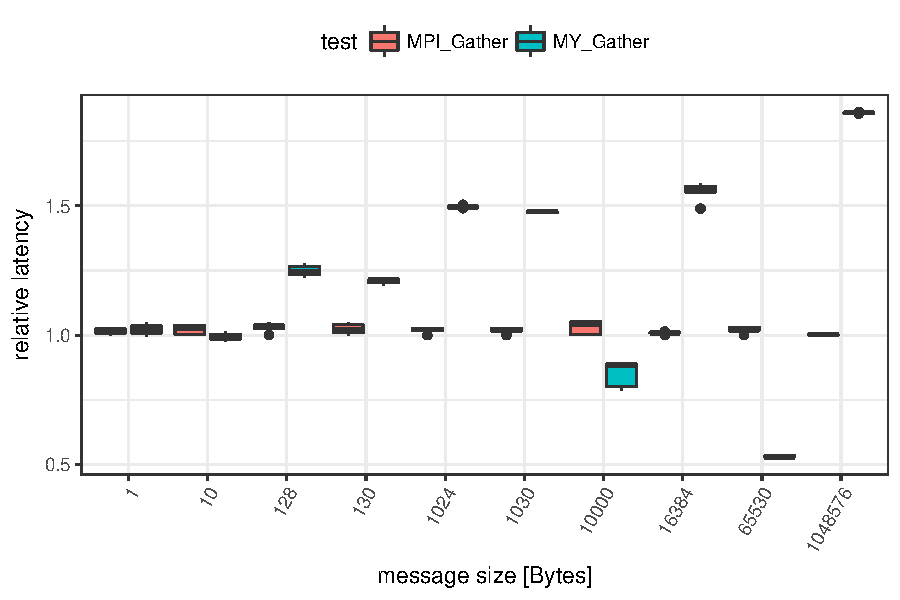
\includegraphics[width=\textwidth]{../benchmarks/mpich/binom/gather_32/rel_runtime.pdf}
        \caption{Relative Runtime with $p=32 \times 16$}
        \label{fig:Gather:MPICH:Rel:32}
    \end{subfigure}
    \begin{subfigure}[b]{0.49\textwidth}
        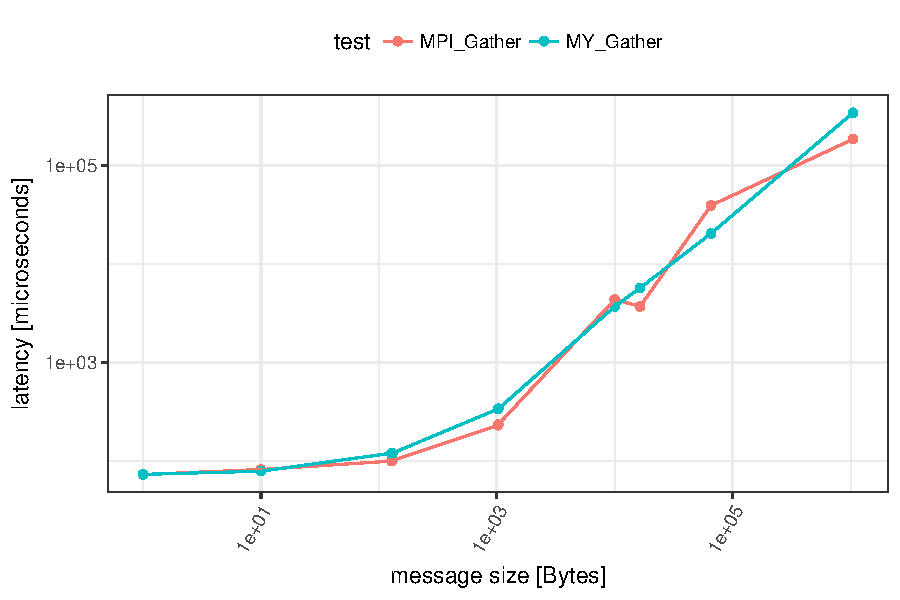
\includegraphics[width=\textwidth]{../benchmarks/mpich/binom/gather_32/runtime.pdf}
        \caption{Absolute Runtime with $p=32 \times 16$}
        \label{fig:Gather:MPICH:Abs:32}
    \end{subfigure}
    
    \caption{\mygather compared to \mpigather of \texttt{MVAPICH2 2.2}}
\end{figure}

%-------
\subsection{Experiments and Discussion -- \myscatter}

\begin{figure}[h]
    \centering
    
    \begin{subfigure}[b]{0.49\textwidth}
        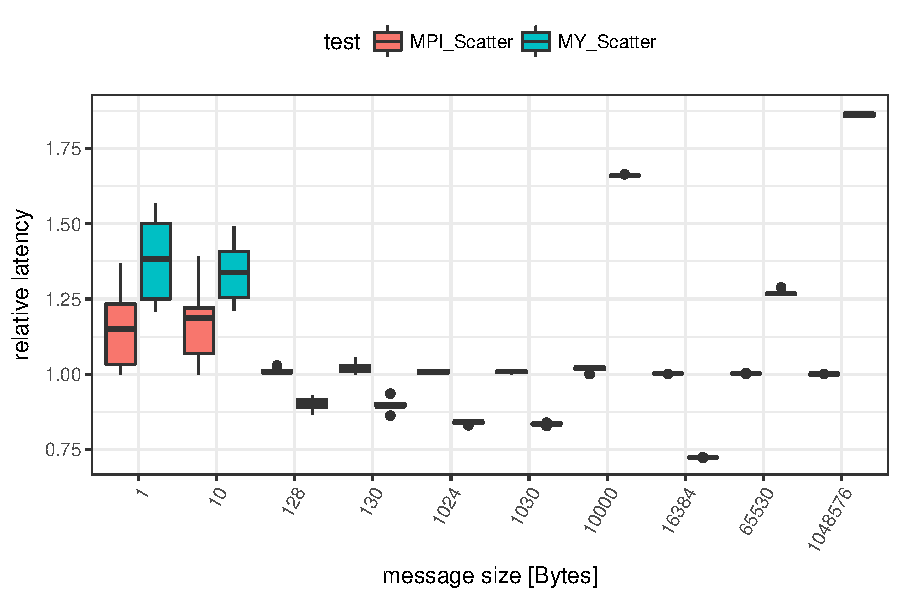
\includegraphics[width=\textwidth]{../benchmarks/openmpi/divide_conquer/scatter_31/rel_runtime.pdf}
        \caption{Relative Runtime with $p=31 \times 16$}
        \label{fig:Scatter:OpenMPI:Rel:31}
    \end{subfigure}
    \begin{subfigure}[b]{0.49\textwidth}
        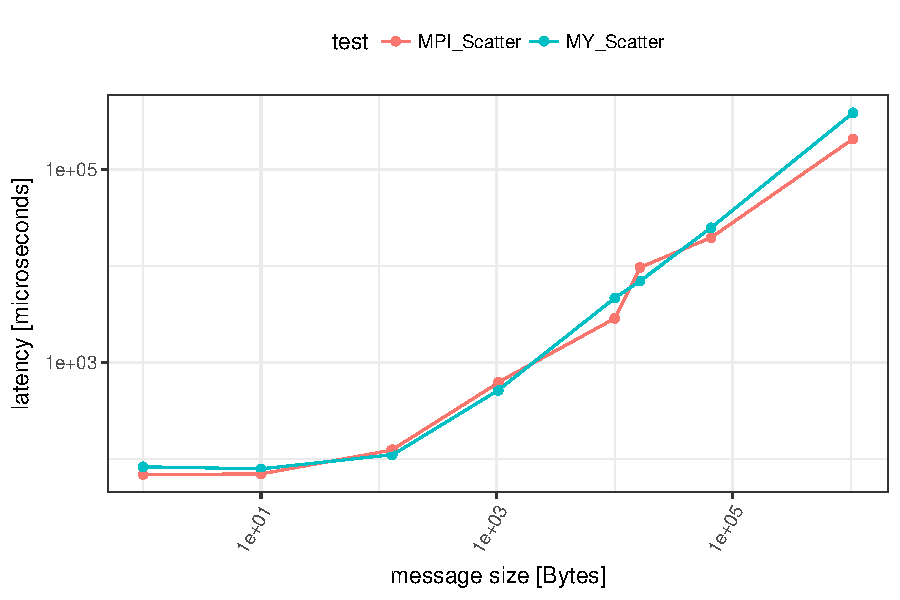
\includegraphics[width=\textwidth]{../benchmarks/openmpi/divide_conquer/scatter_31/runtime.pdf}
        \caption{Absolute Runtime with $p=31 \times 16$}
        \label{fig:Scatter:OpenMPI:Abs:31}
    \end{subfigure}
    
    \begin{subfigure}[b]{0.49\textwidth}
        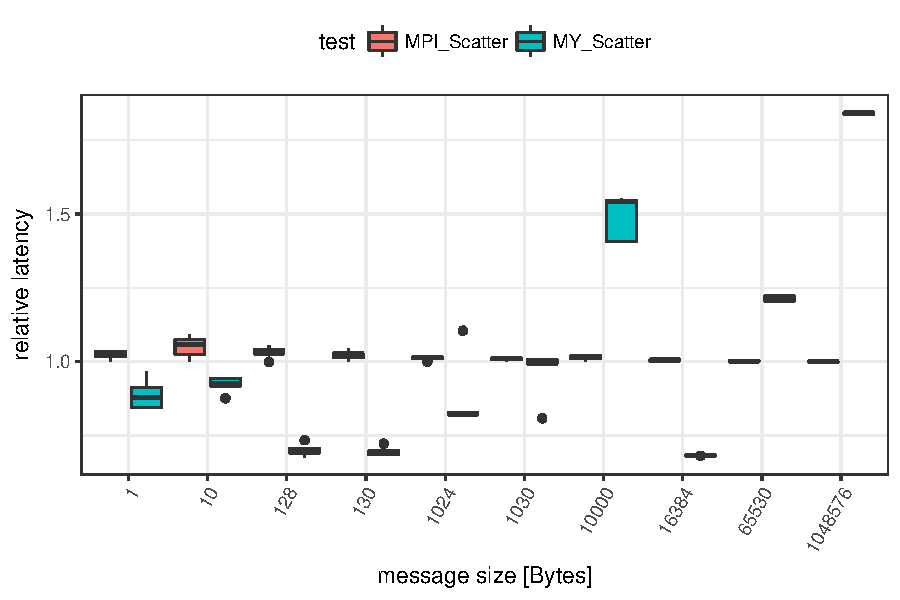
\includegraphics[width=\textwidth]{../benchmarks/openmpi/divide_conquer/scatter_32/rel_runtime.pdf}
        \caption{Relative Runtime with $p=32 \times 16$}
        \label{fig:Scatter:OpenMPI:Rel:32}
    \end{subfigure}
    \begin{subfigure}[b]{0.49\textwidth}
        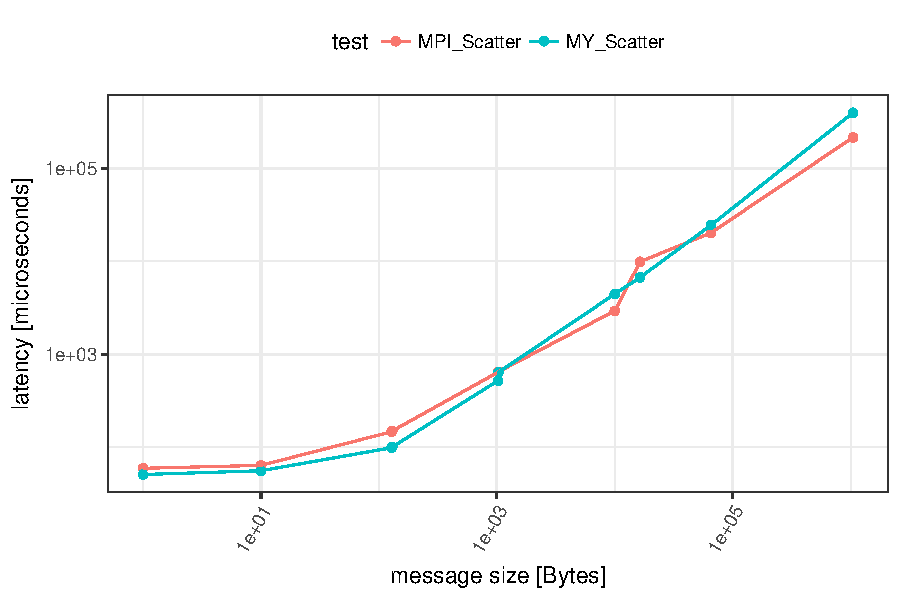
\includegraphics[width=\textwidth]{../benchmarks/openmpi/divide_conquer/scatter_32/runtime.pdf}
        \caption{Absolute Runtime with $p=32 \times 16$}
        \label{fig:Scatter:OpenMPI:Abs:32}
    \end{subfigure}
    
    \caption{\myscatter compared to \mpiscatter of \texttt{Open MPI 1.10.3}}
\end{figure}

\begin{figure}[h]
    \centering
    
    \begin{subfigure}[b]{0.49\textwidth}
        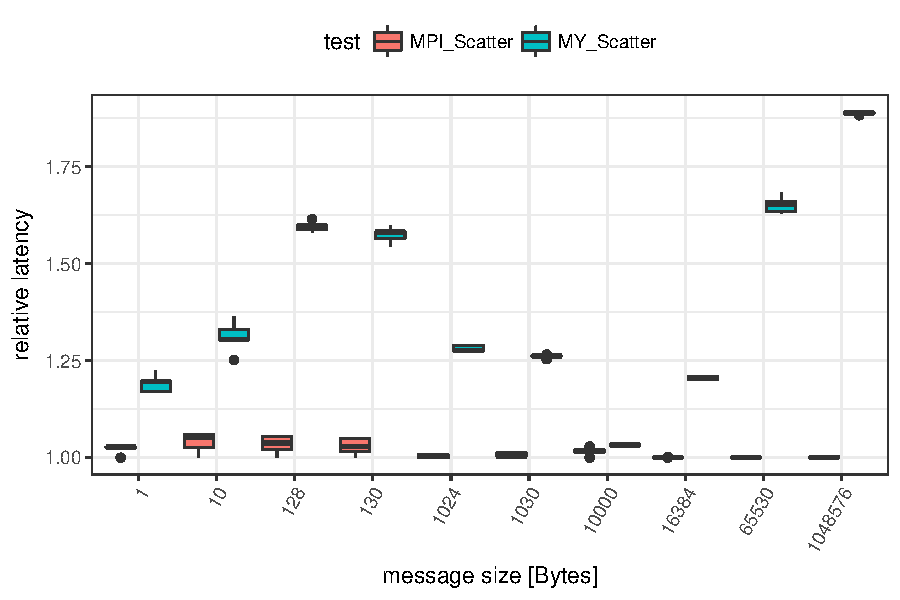
\includegraphics[width=\textwidth]{../benchmarks/mpich/divide_conquer/scatter_31/rel_runtime.pdf}
        \caption{Relative Runtime with $p=31 \times 16$}
        \label{fig:Scatter:MPICH:Rel:31}
    \end{subfigure}
    \begin{subfigure}[b]{0.49\textwidth}
        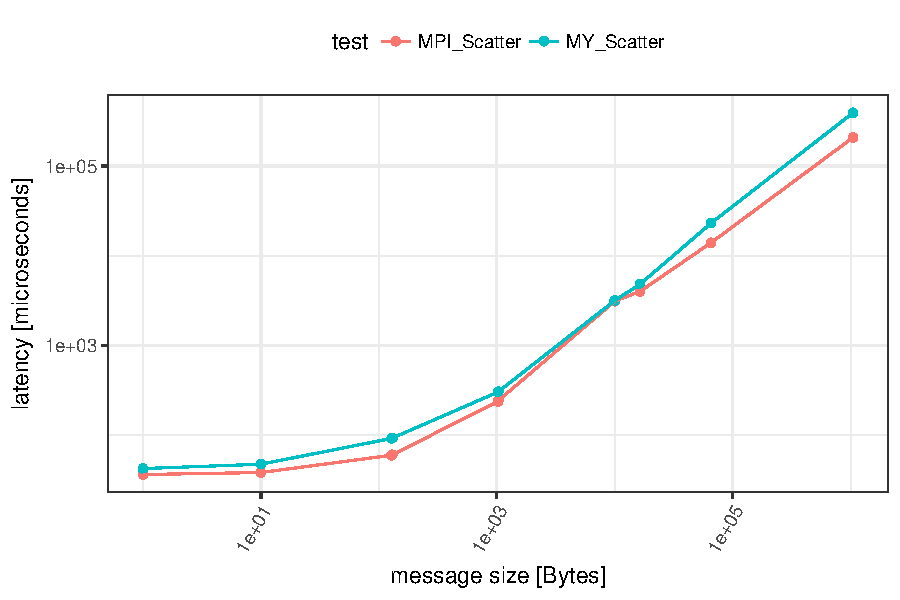
\includegraphics[width=\textwidth]{../benchmarks/mpich/divide_conquer/scatter_31/runtime.pdf}
        \caption{Absolute Runtime with $p=31 \times 16$}
        \label{fig:Scatter:MPICH:Abs:31}
    \end{subfigure}
    
    \begin{subfigure}[b]{0.49\textwidth}
        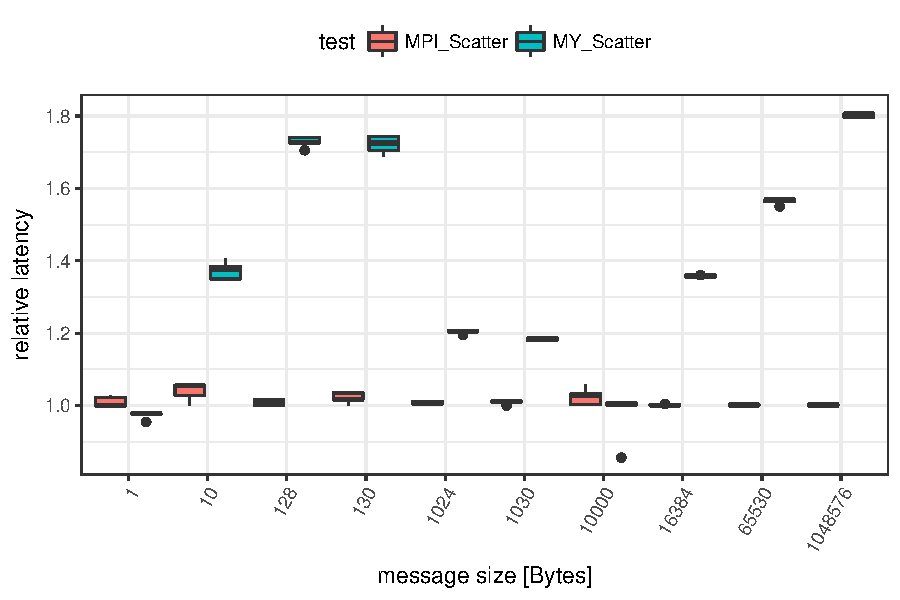
\includegraphics[width=\textwidth]{../benchmarks/mpich/divide_conquer/scatter_32/rel_runtime.pdf}
        \caption{Relative Runtime with $p=32 \times 16$}
        \label{fig:Scatter:MPICH:Rel:32}
    \end{subfigure}
    \begin{subfigure}[b]{0.49\textwidth}
        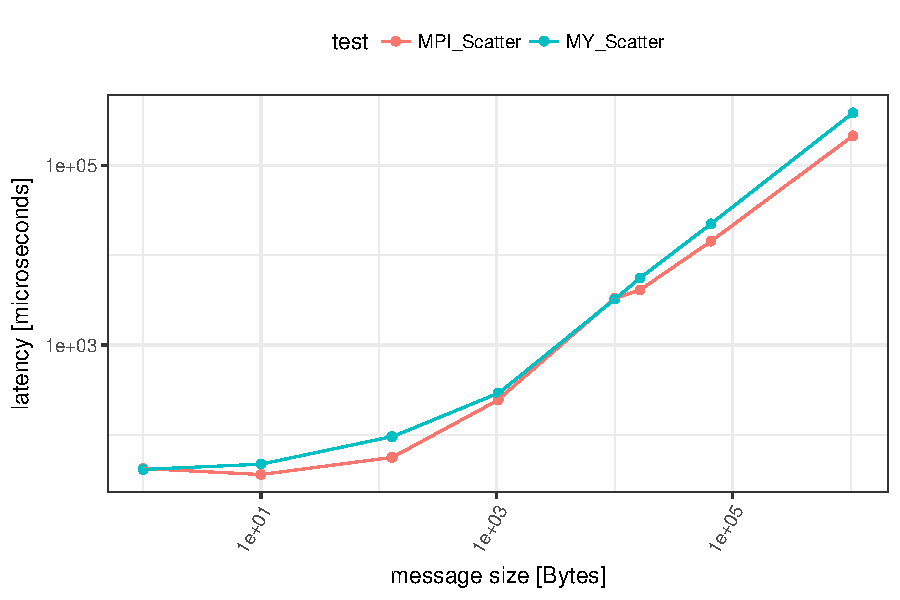
\includegraphics[width=\textwidth]{../benchmarks/mpich/divide_conquer/scatter_32/runtime.pdf}
        \caption{Absolute Runtime with $p=32 \times 16$}
        \label{fig:Scatter:MPICH:Abs:32}
    \end{subfigure}
    
    \caption{\myscatter compared to \mpiscatter of \texttt{MVAPICH2 2.2}}
\end{figure}